\documentclass[a4paper, 12pt]{report}
\usepackage[utf8]{inputenc}
\usepackage[swedish,british]{babel}
\usepackage{graphicx}
\usepackage{fancyhdr}

\usepackage{glossaries}
\pagestyle{fancy}
\begin{document}

\graphicspath{{./images/}}
\title{Smarter and simple Scrabble strategy}
\date{Course: DD143X \\ Supervisor: Johan Boye \\ Kungliga Tekniska Högskolan \\ CSC \\ March 7, 2012}
\author{Frej Connolly \\ Götgatan 78 13TR LÄG1302 \\ 118 30 Stockholm \\ SWEDEN \\ +46(0)73-963 41 90 \\ connolly@kth.se \\
        \and Diana Gren \\ Sköldgatan 8 2TR \\ 118 63 Stockholm \\ SWEDEN \\ +46(0)70-467 47 20 \\ dianagr@kth.se}

\maketitle
\begin{abstract}
The abstract goes here.
\end{abstract}

\selectlanguage{swedish}
\begin{abstract}
Sammanfattning på svenska hamnar här.
\end{abstract}
\selectlanguage{british}
\tableofcontents





\chapter{Introduction}
Scrabble is an old classic game that is fairly easy to learn. However, it is extremely difficult to be a great player. Compared to other classic board games, such as chess, there are more factors to take into consideration when making a move in Scrabble. 

Apart from anagramming and generating words, there are other crucial decisions to make. A player would probably find several legal moves in one round, and then would have to decide which one to place. Choosing the move that generates the highest score is not always the ideal way to go. It could be that making such a move would create a situation in the next round where nothing could be done, or let the opponent score high.

Making the choice of which move to use include many factors, and there are several different techniques and strategies one can follow to make the decision easier. Picking up the bonus squares can generate an extremely high score, hence one strategy is to try to always pick up the bonus squares and prevent the opponent from doing the same. Another way of being successful is to prioritize using letters with high score, since they would not only generate a high total score to the player, but could also create difficult situations in the future if not used as soon as possible.

There are several more possible strategies one can follow, and this study aims to investigate a three of them trying to establish which one is the more rewarding.

\section{Problem statement}
Scrabble requires the players to have a good vocabulary and to become a successful player, some knowledge about how many tiles of each letter is available is preferable. 

When playing, the ability to keep a good balance between consonants and vowels on the rack can profit future moves. Destroying bonus possibilities for the opponent, and at the same time score them oneself is a crucial skill, and experts are probably aware of which tiles have been placed, and those that remain, allowing them to anticipate the future sequence of events. 

\subsection{Question}
Which of the strategies has the most impact on a game? How do the strategies perform against each other, and which one is the most successful one? 


\section {Terminology}
\label{sec:terminology}

\begin{description}
\item{\emph{Anchor square}}: Vacant board square adjacent to a placed tile.

\item{\emph{Bag}} Tiles that have not been drawn by players.

\item{\emph{BOR}}: Balance on rack player.

\item{\emph{BS}}: Bonus square player.

\item{\emph{Cross check set}}: Set of possible letters on an anchor square with regard to adjacent word going vertical from named square.

\item{\emph{DAWG}}: Directed acyclic word graph.

\item{\emph{HSW}}: High score word player.

\item{\emph{Rack}} Tiles on a player's hand. 

\end{description}







\chapter{Background}

\section{Scrabble}
Scrabble was originally created by an american in the 1930s, and arrived in Sweden in 1954 according to Svenska Scrabbleförbundet \cite{forbund}. 

\subsubsection{Components}
Scrabble consists of a 15x15 square board (see appendix section \ref{sec:board}), and a set of letter tiles. Each letter tile has a score associated with it, which depends on which letter is on the tile (see appendix section \ref{sec:letterpoints}). The more difficult letter to use have a higher score, and the more common letters have lower score. The players are given 5 to 8 tiles each, to keep on their \emph{rack}. The game objective is to form words, consisting of at least two letters, using the tiles on the rack and lay out onto the board, horizontally or vertically, and get as high score as possible. 

\subsubsection{Legal move}
There are several alternatives for a player to use a turn. 
\begin{itemize}
\item The player can lay out a legal word onto the board, receiving the corresponding score. After having played a number of tiles, the player draws the same number of new tiles from the bag.
\item The player can pass his turn, receiving zero points.
\item The player can exchange a number of tiles from the rack for the same number of tiles from the bag.
\end{itemize}

Only one of the alternatives can be executed in one round.

\subsubsection{Bonus opportunities}
A small twist in the game is the possibility to generate high scores through the use of bonuses. Dispersed on the board squares, there are four different types of \emph{bonus squares}:

\begin{description}
\item{2L:} Count the score of the letter placed onto this square as double.
\item{3L:} Count the score of the letter placed onto this square as triple.
\item{2W:} Multiply the score of the word by two.
\item{3W:} Multiply the score of the word by three.
\end{description}

The existance of the bonus square makes it possible for the players to receive ver high scores regardless of the length of the word. Strategic placements of letter tiles on these squares can be vital to a player's total score.

In addition to the bonus squares, there is also the possibility to lay out all the tiles from the rack in one move, which will reward the player with 50 points in addition to the word score.

\subsubsection{End of game}
The game ends when a player has emptied the rack, and there are no tiles left in the bag. Also, when there has been a total number of four zero points moves in a row, i.e. the players passed or exchanged tiles.

After the game, all the players still having tils on the rack get a penalty. The sum of the letter scores on the rack is removed from the total score and the winner of the game is the player with the highest score in the end.

\section{Research}
As mentioned above, this is a well studied problem, and many papers and articles are to be found where different problems in the game of Scrabble have been studied. This paper will mostly refer to Appel and Jacobsen \cite{fastest} who discovered a way to represent the dictionary wo that it takes up minimum space in memory.
\begin{figure}[h]
\centering
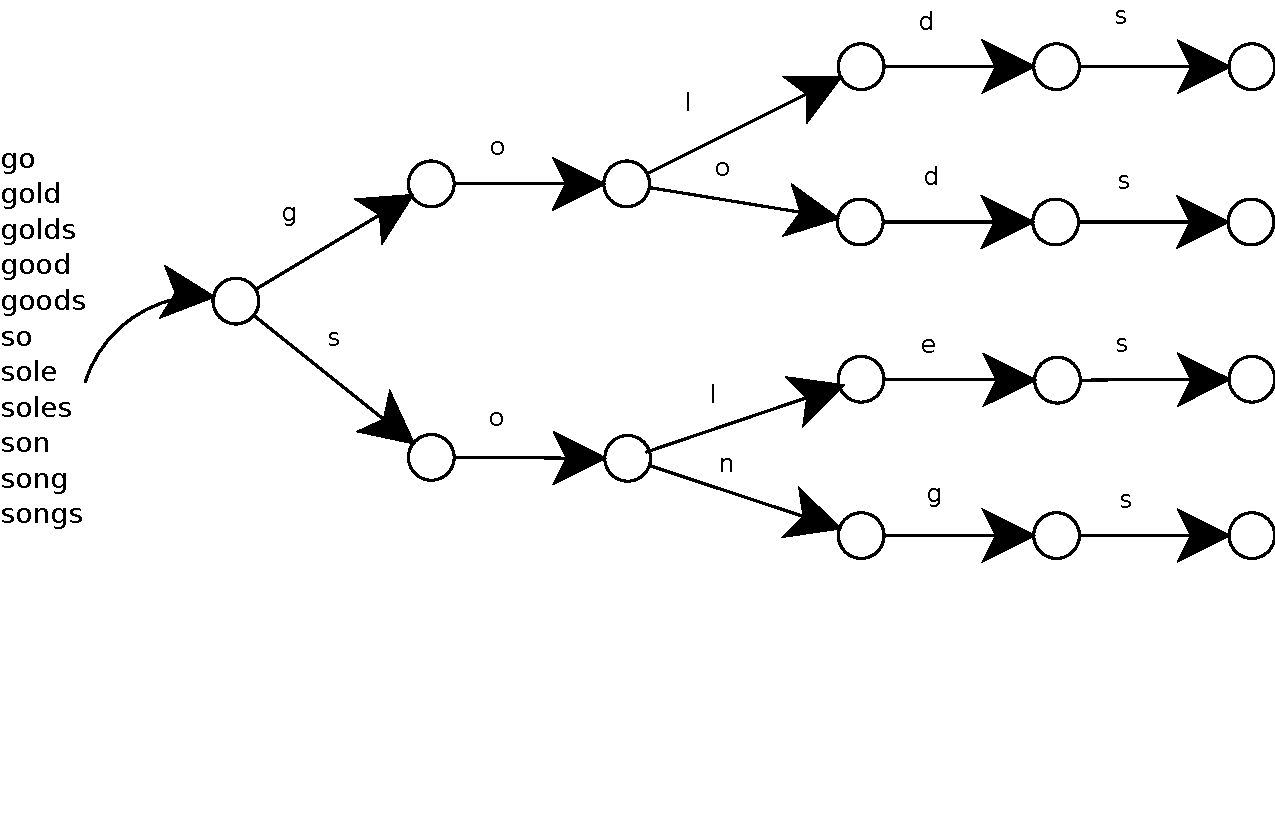
\includegraphics[scale=0.5]{trie}
\caption{Trie. Small dictionary consisting of 11 words represented as a trie.}
\end{figure}
\subsection{Dictionary}
Appel and Jacobsen \cite{fastest} came to the conclusion that a word search will be incredibly fast in a \emph{Directed Acyclic Word Graph}, which in this study will be referred to as a \emph{DAWG}. A DAWG is generally built from a trie, and can be explaind like a minimized trie. Where a trie has a lot of redundancy, becuase of edges and nodes being identical, no such thing occurres in a DAWG. All the identical edges and nodes are removed, and reduced to only one occurancy. As an example in the paper mentioned, the dictionary consisting of more than 100 000 words taking up a memory space of a half mega bytes, could be reduced to occupy only 175 kile bytes.


\subsection{Word generation}
The problem of generating legal moves can be reduces to one dimension. Instead of doing a search in two directions (up and right) it is possible to use an algorithm that generates words only horizontally. The argument is that generating a word vertically is basically the same thing as generating a word horizontally. The only difference is that the board is transposed. Therefore, the algorithm to generate words is limited to only generate horizontally, and for each move we do two searches, where one is over the transposed board.

\subsubsection{Anchor squares}
A key in the algorithm implemented are the \emph{anchor squares}, which are the empy squares next to a non-empty square as can be seen in figure \ref{fig:anchors}. These are important since words can only be built from already existing tiles. In the very forst move there is only one anchor; the center square, since the player making the first move always has to start in the center square.

\begin{figure}[h]
\centering
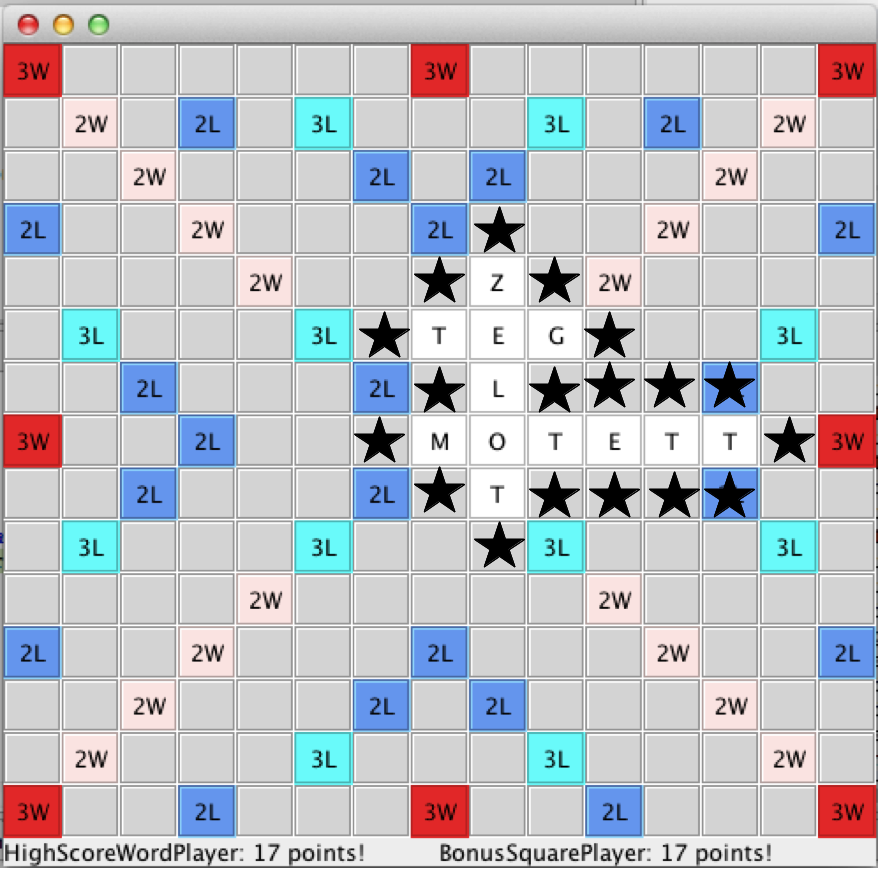
\includegraphics[scale=0.5]{anchors}
\caption{Anchor squares. The adjacent tiles are the anchor tiles from which the word generation begins.}
\label{fig:anchors}
\end{figure}

\subsubsection{Cross-check sets}
When placing a word horizontally, the vertically placed letters also have to create a legal word. It is quite easy to establish that if we place a word horizontally, the vertical word can increas with only one letter at a time. This makes it possible to calculate, for each anchor square, which set of letters that are possible to place at that square. The calculations can be made before each move, and allows the player to place a word by row, without considering the rest of the board. The set of available letter for one square is in Appel and Jacobsen's paper \cite{fastest} referred to as a \emph{cross-check set}

\subsection{Game strategies}
\label{sec:strategies}
If one is a beginner at Scrabble, there are meny small tricks to learn to advance quickly. Some of the tricks can be listed as:

\begin{itemize}
\item Difficult letters. Letters with high score are usually more difficult to place and should be used as soon as possible.
\item Balance on the rack. It is easy to get stuck with only consonants or only vowels on the rack, keeping a good balance can therefore be a good idea to avoid deadlocks in the future.
\item Bonus squares. Hitting the bonus squares can generate a high score. Although it is preferable to avoid opening opportunities for the opponent to do the same.
\item Word extensions. According to Sheppard \cite{perfectgame}, the ability to find extensions (i.e. prefixes and suffixes) to already placed words, is a key to being a successful player since such moves can generate very high scores.
\item Vocabulary. There are many short words in the language, and it is instantly rewarding if a player can learn many short word letters.
\end{itemize}






\chapter{Implementation}
The study is based on an implementation that follows the example of Appel and Jacobsen \cite{fastest}, with some small modifications. Since implementing a DAWG seemed like a time consuming project, a chioce was made to stay with the trie. The advantage with a DAWG is that it saves a lot of memory, but there were no problems with memory space, and therefore an unnecessary thing to focus on.

In the implementation there were some game limitations made to make the study fit into the given time span. The game limitations are described in section \ref{sec:limitations}.

Three different agents were implemented with different strategies to follow and they are all described in section \ref{sec:agents}.

The analysis and the final results are shown in section \ref{sec:analysis}.

\section{Game limitations}
\label{sec:limitations}
To limit the work load to fit into the time span, some limitations were made to the game. This study focuses on games played by only two players, and the implementation is therefore customized to handle only two player games. The players have two options during a turn; either lay a word, or pass the turn and receieve zero points. In other words; the possibility to change tiles if no word can be found is removed. 

The bag is also minimized, and do not contain any blank letters or other special tiles that are not letters. The result is that a Q or a W never can be used. In addition, the game is played in Swedish by the agents.

\section{Agents}
\label{sec:agents}
To see which of the very basic strategies listed in section \ref{sec:strategies} is the most successful one against the others, three agents with different strategies were implemented. The would play against each other in order to generate results for later analyze. This section describes the three different agents implemented, and their strategy in the game. In order to evaluate which strategies are the more rewarding, the agents are implemented with only \emph{one} strategy. An agent who calculates the total score of a move and chooses the highest one will easily win over the tested agents in this study. The agents will be referred to as the HSW player, the BS player and the BOR player (see section \ref{sec:terminology}).

\subsection{High Score Word player}
One strategy one can use when playing Scrabble is the fact that some letters are more worth than others. These letter are less commonly used in the language and is therefore more difficult to use. Naturally, one would want to use them as soon as there is an opportunity, to not risk getting stuck later in the game. One od the agents tested in this study follows the strategy of placing higher score generating letters first. By all legal moves generated, the agent will chose the one were the word itself has the highest score. 

\subsection{Bonus Square player}
Sometimes, it can be more rewarding to place a relatively short word than a longer one. This is because of the bonus squares spread out on the board. The can multiply the value of either one letter, or the entire word placed, and can therefore generate quite high scores. The second agent strives to place words over bonus squares, to hopefully generate a high score. If there are several opportunities to reach a bonus tile, the most rewarding one is chosen by the agent, i.e. the word reaching the bonus square with the highest bonus.

\subsection{Balance On Rack player}
An important thing to think about when playing Scrabble is to plan for the next move. If a player ends up with only consonants on the rack, the possibility of laying out a word is reduced. The third agent tested tries to always keep a good balance between vowels and consonants on the rack, to avoid deadlocks later in the game. The agent knows the \emph{ideal ratio} and tries to lay out words so that the words left on the rack returns a ratio as close to the ideal ratio as possible. Tests with different ideal ratios are made.

\chapter{Results}
\label{sec:analysis}
Each of the agents has been tested against the others, to let us evaluate the impact of each strategy. Explanations of the agents can be read about in section \ref{sec:agents}. Section \ref{sec:conditions} describes under which conditions the tests were made.

Sections \ref{sec:highBalance}, \ref{sec:balanceBonus} and \ref{sec:bonusHigh} show the results from each run.
 
\section{Test conditions}
\label{sec:conditions}
\subsection{Games}
In one run the agents were set to play 1000 games against each other and to minimize the impact of opening the game in the results, both agents started the game 500 times. Each run were made 10 times, so the total result is based on 10 000 games. It was established that there were no significant changes in the results between running 1000 games, and 10 000 games, and would therefore probably be reduntant to make more tests. 

\subsection{Dictionaries}
Two dictionaries were used in the tests; one consisting of only the normal form of each word and the other consisting of all possible forms of each words, where the latter is a set of 480391 words. The former consists of 83247 words. The rules of Swedish Scrabble do not allow words of all forms, but the english does. Therefore, it seemed interesting to compare how the agents would perform with different conditions. There could be situations where for instance the bonus player has an advantage if conjunctions are allowed, since it strives always after covering the bonus squares. The large dictionary could allow the player to place short extensions to already placed words.

The longest word in the used dictionary is ammoniumdiamintetrakistiocyanatokromat. The shortest possible word to place on board is all two letter words in the dictionary \cite{dictionary}. The number of two letter words is 121. Table \ref{table:dictionary+length}.
\begin{table}[h]
\centering
	\begin{tabular}{l | c | c}
	& Base words & All words \\
	\hline
	Mean & 9.5 & 11.2 \\
	\hline
	Longest & \multicolumn{2}{c}{ammoniumdiamintetrakistiocyanatokromat} \\
	\hline
	Shortest & \multicolumn{2}{c}{121 two letter words} \\ 
	\end{tabular}
\caption{Mean, largest and smallest lengths of legal words in the dictionary.}
\label{table:dictionary+length}
\end{table}

\section{High score words vs Balance}
\label{sec:highBalance}

The results from runs over the large dictionary and the small dictionary do not differ that much, as can be seen in figure \ref{fig:smallDict} and figure \ref{fig:bonusBalanceLargeDict}.
The BOR player uses a ratio between vowels and consonants on the rack, and strives to keep the ratio after each move. The wanted number of vowels on hand will be referred to as \emph{vowel ratio}. Several tests were made with the BOR player to see if there is any difference when altering the ratio parameter. The ratio is calculated as the number of vowels left on hand divided into the number of consonants left on hand. Table \ref{tab:bor+hsw} shows the results of the runs made with different ideal number of vowels on hand.

\begin{table}[h]
\centering
    \begin{tabular}{ l | l | l }
   	& BOR & HSW \\
   	\hline
   	Wins & 1 & 9999 \\
	Draws & 0 & 0 \\
	Wins when started playing & 0 & 5009 \\   	
	Mean score & 124 & 420 \\
	Median score & 123 & 415 \\	 	 
	Highest score & 299 & 745 \\
	Lowest score & -16 & -12 \\		
    \end{tabular}
\caption{Result from 10 000 games with vowel ratio 1/8 and words in all inflection forms from the Swedish dictionary (480 391 words).}
\label{table:borhswstats}
\end{table}

\begin{table}[h]
\centering
    \begin{tabular}{ l | l | l }
   	& BOR & HSW \\
   	\hline
   	Wins & 1206 & 8762 \\
	Draws & 32 & 32 \\
	Wins when started playing & 643 & 4431 \\   	
	Mean score & 214 & 309 \\
	Median score & 213 & 307 \\	 	 
	Highest score & 407 & 624 \\
	Lowest score & -9 & -19 \\		
    \end{tabular}
\caption{Result from 10 000 games with vowel ratio 8/8 and words in all inflection forms from the Swedish dictionary (480 391 words).}
\label{table:borhswstats}
\end{table}

The results show that the HSW player is generally more successful playing the game. The BOR player does not take the word score in consideration when playing, but only the ratio, and it it obviously not the most rewarding strategy to follow. An interesting observation is that if the BOR agent tries to keep a ratio of vowels close to 1, i.e all tiles being vowels, there is a significant peak in the number of winning games for the agent. On the other hand, trying to keep one vowel on hand after each round seems to not be as smart, since the agent lost almost 100\% of all games.

\begin{table}[h]
\centering
    \begin{tabular}{ | c | c | c | p{5cm} |}
    \hline
   	Vowel ratio & HSW wins & BOR wins \\ \hline
	0/8 & 9922 & 73 \\ \hline
    	1/8 & 9999  & 1 \\ \hline
    	2/8 & 9484 & 507 \\ \hline
    	3/8 & 9777 & 212 \\ \hline
	4/8 & 9735 & 262 \\ \hline
	5/8 & 9627 & 368 \\ \hline
	6/8 & 9146 & 838 \\ \hline
	7/8 & 9863 & 134 \\ \hline
	8/8 & 8762 & 1206 \\ \hline
    \end{tabular}
\caption{Winnings depending on vowel ratio. Amount of winning games of a total of 10 000 games.}
\label{tab:bor+hsw}
\end{table}


\section{Balance vs Bonus}
\label{sec:balanceBonus}
The BOR player continues to perform doubtly against the BS player. Also here the BS player consideres what bonus it will be given in a certain move, and chooses the highest one. Naturally the BOR player that only cares about its ratio on the rack will perform worse. The results from runs with different vowel ratio in the BOR player can be seen in table \ref{tab:bor+bs}.

Note that the BOR player is stable with its game results. In figure \ref{fig:bonusBalanceLargeDict} one can see that the BS player in some games made an extremely poor performance, receiving zero points or less, while the BOR player keeps the graph quite thin, i.e. the results differ less from game to game.

\begin{table}[h]
\centering
    \begin{tabular}{ | c | c | c |  p{5cm} |}
    \hline
   	Vowel ratio & BS wins & BOR wins \\ \hline
	0/8 & 9925 & 72 \\ \hline
    	1/8 & 9987 & 12 \\ \hline
    	2/8 & 9670 & 325 \\ \hline
    	3/8 & 9829 & 165 \\ \hline
	4/8 & 9818 & 172 \\ \hline
	5/8 & 9731 & 261 \\ \hline
	6/8 & 9370 & 620 \\ \hline
	7/8 & 9859 & 141 \\ \hline
	8/8 & 9074 & 915 \\ \hline
    \end{tabular}
\caption{Winnings depending on vowel ratio. Amount of winning games of a total of 10 000 games.}
\label{tab:bor+bs}
\end{table}




\section{Bonus vs High score words}
\label{sec:bonusHigh}
\emph{BS} wins just over 6 of 10 times against \emph{HSW} when using all inflection forms from the Swedish dictionary table \ref{table:bs+hsw+allwords} and well over 5 of 10 times when only the base forms of words is used table \ref{table:bs+hsw+baseforms}. When \emph{BS} started playing it won 52\% of its wins when using all inflection forms. For \emph{HSW} 53\% of its wins. When using only the base form both of them were winning 51\% its wins when started laying out words.

The resulting mean, median, highest and lowest scores is significant higher when using all inflection forms. Lowest score is negative for both players when using only base forms. \emph{BS} mean score is 24\% higher in table \ref{table:bs+hsw+allwords} compared to table \ref{table:bs+hsw+baseforms}. The same applies for the end score which is higher when using all words Appendix Figure \ref{fig:bs+hsw+totalscores}.

\begin{table}[h]
\centering
    \begin{tabular}{ l | l | l }
   	& Bonus Squares & High score words \\
   	\hline
   	Wins & 6104 & 3857 \\
	Wins when started playing & 3148 & 2040 \\   	
	Mean score & 308 & 278 \\
	Median score & 301 & 273 \\	 	 
	Highest score & 724 & 606 \\
	Lowest score & 85 & 61 \\		
	\hline 
   	Draws & 39 & 39 \\
    \end{tabular}
\caption{Result from 10 000 games with words in all inflection forms from the Swedish dictionary (480 391 words).}
\label{table:bs+hsw+allwords}
\end{table}

\begin{table}[h]
\centering
    \begin{tabular}{ l | l | l }
   	& Bonus Squares & High score words \\
   	\hline
   	Wins & 5427 & 4521 \\
	Wins when started playing & 2758 & 2314 \\   	
	Mean score & 248 & 240 \\
	Median score & 246 & 234 \\	 	 
	Highest score & 488 & 506 \\
	Lowest score & -15 & -11 \\		
	\hline 
   	Draws & 52 & 52 \\
    \end{tabular}
\caption{Result from 10 000 games with only words in base form from the Swedish dictionary (83 247 words).}
\label{table:bs+hsw+baseforms}
\end{table}

\chapter{Conclusions}
\section{Discussions}
\subsubsection{BOR player}
The BOR player is significantly better with a vowel ratio of 8/8. It can probably be explained from the fact that when choosing a move, and the vowel ratio is 8/8 (1) it is easier for the agent to place longer words. Imagine the agent placing a word using all tiles but one, and the remaining tile on hand is a vowel. This would be a preferable move if the ratio is 1, but not if the ratio is less. If the ratio would be 4/8 for example, the agent would choose a move that leaves two tiles, where one is a vowel, over the move with a longer word. 

\subsubsection{HSW player}
High score word player conclusions go here.

\subsubsection{BS player}
Choosing to place words that will occupy a bonus square is rewarding. It will not only give a high score but will also destroy the possiblity for the opponent to reach a bonus square.

It has active playing style with the mission to conquer the bonus squares at all cost. With the power of a big dictionary it will have a higher probability to reach a bonus. It is easy to extend words already on board when having the possibility to use all inflection forms of words. The end score will also be higher Figure \ref{fig:bs+hsw+totalscores}. When using only base words it will struggle to find bonus squares. This is due to 

\section{Conclusions}


\appendix
\chapter{Game conditions}
\graphicspath{{images/}}

\section{Board}
\label{sec:board}
\begin{figure}[h]
\centering
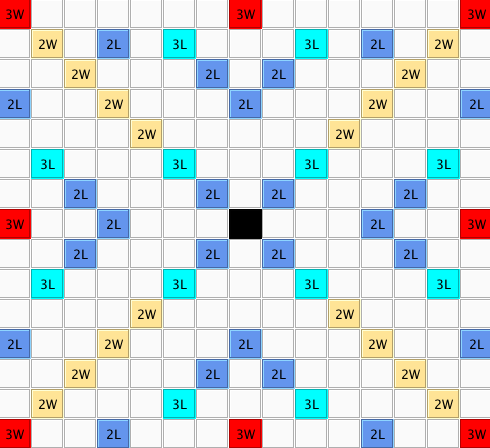
\includegraphics[scale=0.5]{board}
\caption {Game board. 15x15 square board with bonus squares.}
\label{fig:board}
\end{figure}

\section{Letter points}
\label{sec:letterpoints}
\begin{itemize}
	\item{\emph{1 point}} \textbf{A}x8, \textbf{D}x5, \textbf{E}x7, \textbf{I}x5, \textbf{L}x5, \textbf{N}x6, \textbf{R}x8, \textbf{S}x8, \textbf{T}x8
	\item{\emph{2 points}} \textbf{G}x3, \textbf{H}x2, \textbf{K}x3, \textbf{M}x3, \textbf{O}x5
	\item{\emph{3 points}} \textbf{F}x2, \textbf{V}x2, \textbf{Å}x2
	\item{\emph{4 points}} \textbf{B}x2, \textbf{P}x2, \textbf{U}x3, \textbf{Ä}x2, \textbf{Ö}x2
	\item{\emph{7 points}} \textbf{J}x1, \textbf{Y}x1
	\item{\emph{8 points}} \textbf{C}x1, \textbf{X}x1
	\item{\emph{10 points}} \textbf{Z}x1
\end{itemize}


\chapter{Diagrams}
\graphicspath{{../results/Plots/}}

\begin{figure}[h]
\centering
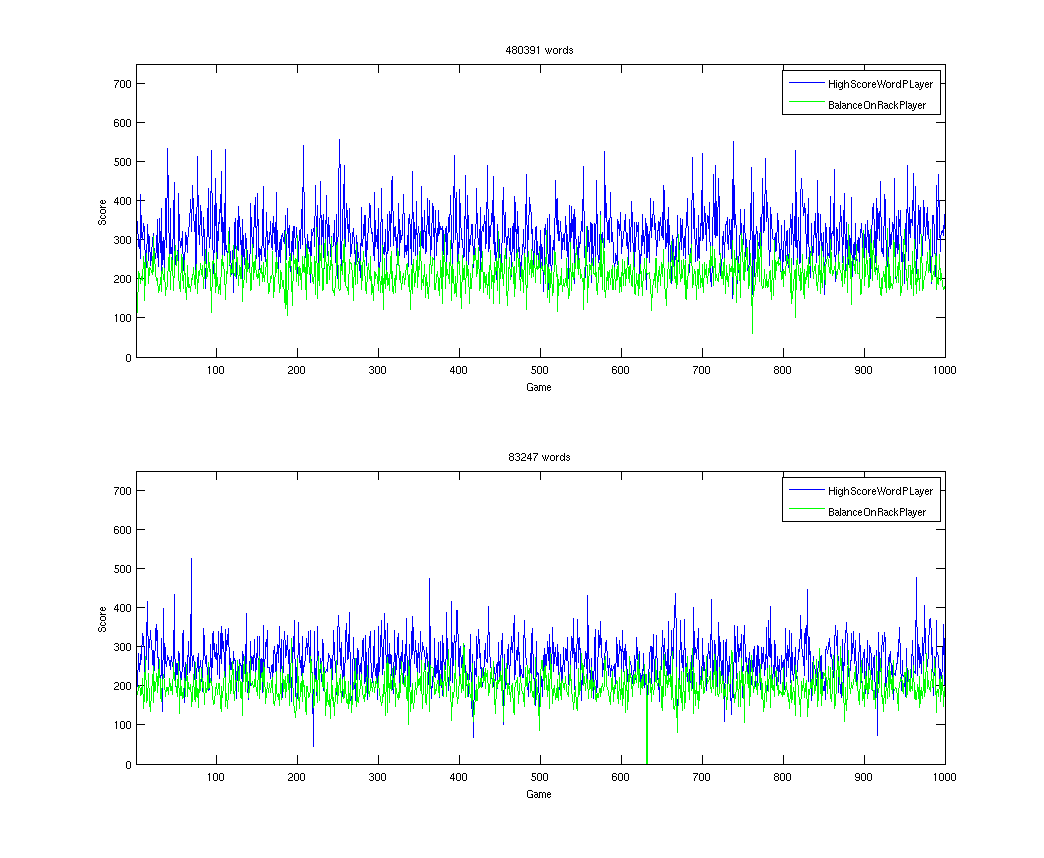
\includegraphics[scale=0.5]{HighBalance8vow_bothDict}
\caption {Scores with vowel ratio 8/8. Scores of the two players in 1000 games with 83 247 words available.}
\label{fig:smallDict}
\end{figure}

\begin{figure}[h]
\centering
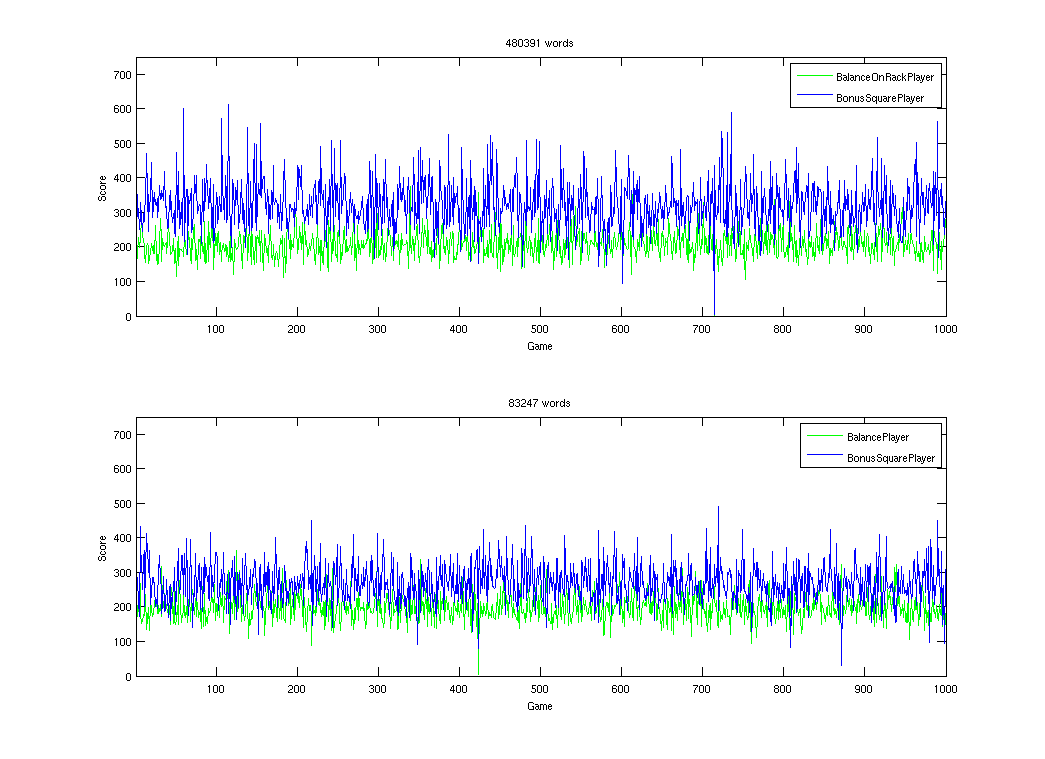
\includegraphics[scale=0.5]{BonusBalance8vow_bothDict}
\caption {Scores with vowel ratio 8/8. Scores of the two players in 1000 games with 480 391 words available.}
\label{fig:bonusBalanceLargeDict}
\end{figure}

\begin{figure}
\centering
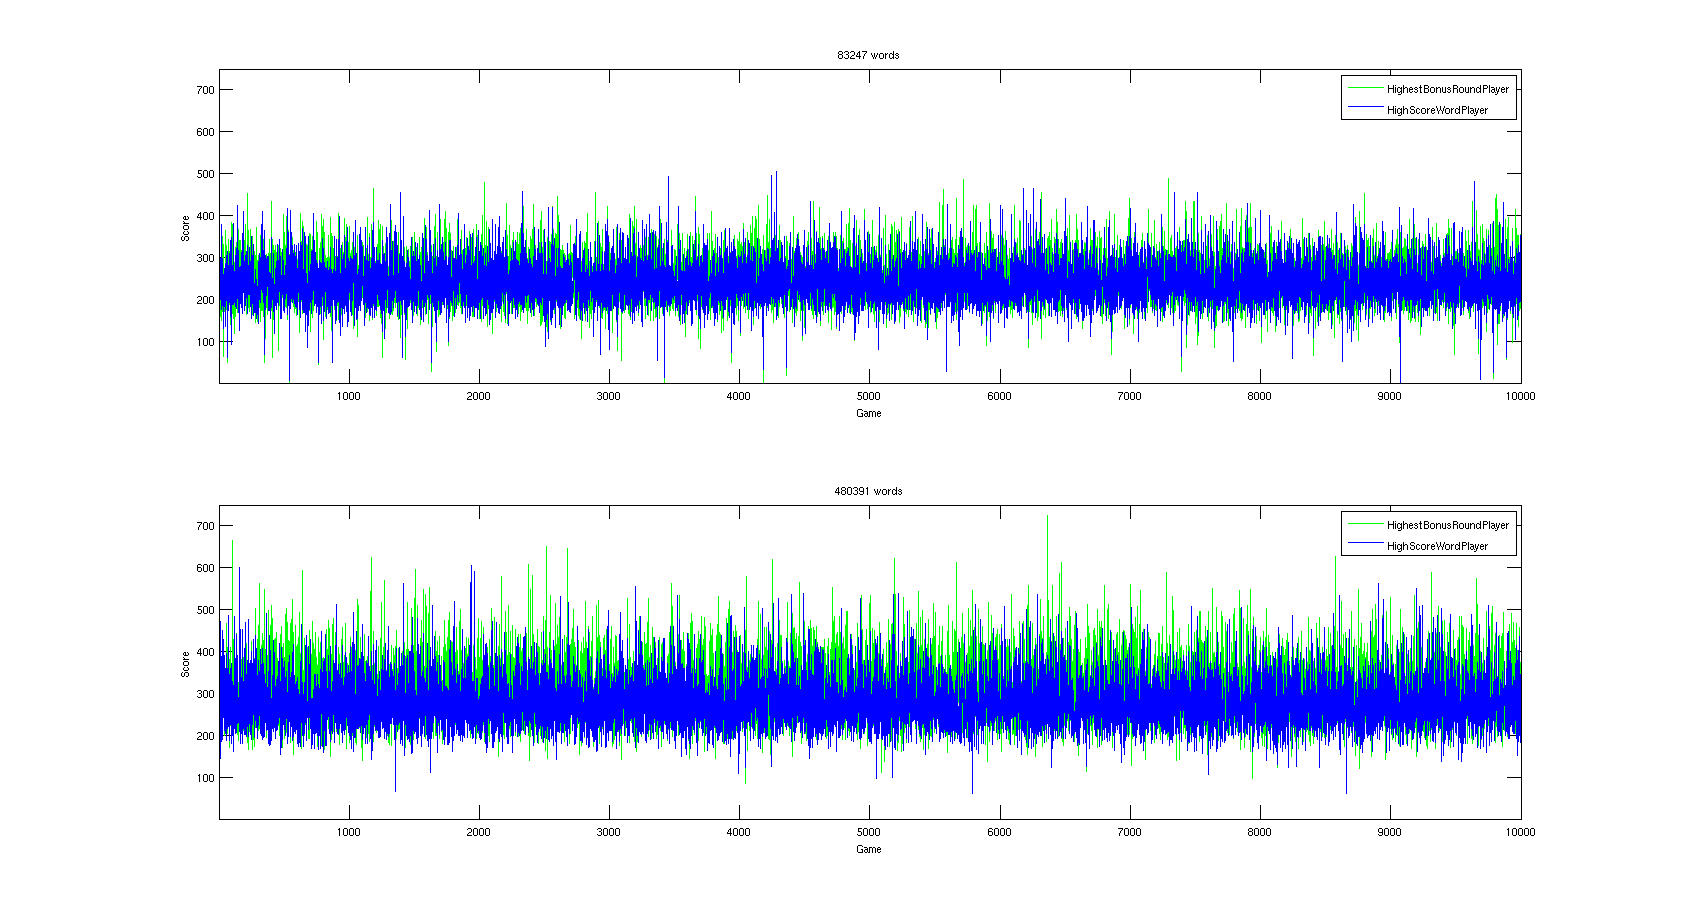
\includegraphics[scale=0.3]{Highest_Bonus_Round_vs_High_Score_Word_10000}
\caption {End scores of the two players in 10000 games. Upper graph with base words only and lower graph with all inflection forms.}
\label{fig:bs+hsw+totalscores}
\end{figure}



\begin{thebibliography}{100}  
  \bibitem{perfectgame} Sheppard, B., 2002, Towards Perfect Play of Scrabble, Maastricht.
  \bibitem{fastest} Appel A. W., Jacobson, G. J., 1985, The World’s Fastest Scrabble Program, Commun. ACM, 31(5), 572-585, May 1988.
\bibitem{faster} Gordon, S. A., 1993, A Faster Scrabble Move Generation Algorithm, Software - Practice and experience, Vol. 24(2), 219-232, February 1994.
\bibitem{quakle} Katz-Brown, J., O’Laughlin, J., Fultz, J., Liberty, M., Buddhdev, A., 2006, Quakle - open source crossword game software, http://people.csail.mit.edu/jasonkb/quackle/, 2 January 2012,  12 February 2012.
\bibitem{scrabblewiki} Wikipedia, Scrabble, http://en.wikipedia.org/wiki/Scrabble, 12 February 2012.
\bibitem{frank} Andersson, G., Ivansson, L., Frank - crossword software game, http://ivansson.org/Frank/, 22 August 2009, 12 February 2012.
\bibitem{wordfeud} Hbwares, Wordfeud, http://www.wordfeud.com, September 2010, 12 February 2012.
\bibitem{ai} Russell S., Norvig P. Artificial Intelligence: A Modern Approach 3rd ed. Prentice Hall. 2009
\bibitem{inforetrieve} Manning C. D., Raghavan P., Schütze H., Introduction to Information Retrieval, Cambridge University Press, 2008, p. 49-65.
\bibitem{forbund} Svenska Scrabbleförbundet, www.scrabbleforbundet.se.
\bibitem{dictionary}Den stora svenska ordlistan, http://code.google.com/p/dsso/downloads/detail?name=dsso-1.52.txt\&can=1\&q=
\end{thebibliography}
\end{document}